\documentclass[preprint,11pt,authoryear]{elsarticle}

\usepackage[T1]{fontenc}
\usepackage[utf8]{inputenc}
\usepackage{lmodern}
\usepackage{amsmath,amssymb,bm}
\usepackage{graphicx}
\usepackage{booktabs,tabularx,array}
\usepackage{rotating}
\usepackage{microtype}
\usepackage{lineno}
\usepackage[a4paper,left=1.55cm,right=1.55cm,top=1.70cm,bottom=1.70cm]{geometry}
\usepackage[dvipsnames]{xcolor}
\usepackage[colorlinks=true,linkcolor=MidnightBlue,citecolor=MidnightBlue,urlcolor=MidnightBlue]{hyperref}

\modulolinenumbers[5]
\graphicspath{{figures/}}
\setlength{\textfloatsep}{11pt plus 2pt minus 2pt}
\setlength{\floatsep}{9pt plus 2pt minus 2pt}
\setcounter{topnumber}{3}
\renewcommand{\topfraction}{0.92}
\renewcommand{\textfraction}{0.06}
\renewcommand{\floatpagefraction}{0.82}

\begin{document}

\begin{frontmatter}
\title{GEL-Ped: Geometry-encoded learning for pedestrian forecasting under limited data and unseen flow topology}
\author[melb]{Amir Ghorbani\corref{cor1}}
\cortext[cor1]{Corresponding author}
\ead{ghorbania@student.unimelb.edu.au}
\affiliation[melb]{organization={Transport Engineering Group, Department of Infrastructure Engineering, The University of Melbourne},addressline={Grattan Street},city={Parkville},state={VIC},postcode={3010},country={Australia}}
\begin{abstract}
Reliable pedestrian forecasts must support decisions when local flow patterns and the amount of available site data differ from model development. Purely neural predictors can interpolate familiar scenes well, while mechanism-based models offer structure but often sacrifice flexibility. We introduce \textbf{GEL-Ped} (\textbf{G}eometry-\textbf{E}ncoded \textbf{L}earning for \textbf{Ped}estrian Forecasting), a dual-expert predictor that combines an unrestricted neural branch with a route-aligned tensor-residual branch. The structured branch encodes progress and lateral avoidance separately and uses an observable support gate; complete-run validation selects the blend without using external test scenes. We evaluate the resulting model on controlled corridor, altered-geometry, and perpendicular-crossing experiments against operational, linear, neural, and goal-stable hybrid references. GEL-Ped does not replace the direct network for well-sampled familiar-scene interpolation. Its benefit appears when interaction topology changes or site-specific fitting data are restricted, where the directional prior improves transfer consistently across forecast horizons. The study therefore provides an evidence-based model-selection rule and a reproducible framework for testing when physical structure adds practical value to pedestrian prediction.
\end{abstract}
\begin{keyword}
pedestrian dynamics \sep trajectory prediction \sep data efficiency \sep cross-topology transfer \sep physics-guided learning \sep social interaction \sep hybrid prediction
\end{keyword}
\end{frontmatter}
\linenumbers

\section{Introduction}

Pedestrian forecasts are increasingly part of operational systems rather than isolated academic benchmarks. A station-monitoring system may need to anticipate local conflicts, a mobile platform must update nearby motion before selecting a path, and a digital representation of a facility must respond when demand or directional flow changes. In each case, short-horizon prediction sits between trajectory sensing and a downstream decision. The model must therefore be accurate, fast enough for repeated use, and credible outside the precise runs on which it was calibrated.

The main modelling choice is often presented as a contest between mechanism and learning. Mechanistic models express desired motion, interpersonal repulsion, anticipation, or collision avoidance through a small set of understandable terms \citep{helbing1995,moussaid2011,karamouzas2014,xu2021}. Neural trajectory models instead learn interaction and temporal representations from data and have achieved strong results in matched-scene forecasting \citep{alahi2016,mohamed2020,salzmann2020,su2024}. Neither family automatically solves the operational problem. A compact model can be interpretable but inaccurate; a neural model can be accurate but data-hungry or sensitive to a change in interaction topology. Interpretability alone is not a sufficient reason to accept worse predictions.

Recent work has begun to bridge the two families. Goal-stable dynamics can constrain a Transformer toward an estimated destination \citep{wang2024dynamics}, interpretable interaction learning can expose heterogeneous social responses \citep{liu2024}, data-driven inference can recover effective pedestrian dynamics \citep{pouw2024}, and differential constraints can regularize probabilistic forecasts \citep{sang2024}. Other hybrids update route and speed modules online \citep{mai2025} or combine learned state recognition with movement strategies for dense pushing behaviour \citep{xu2026}. These studies establish that hybrid learning itself is not a research gap. What remains unclear is whether an explicit longitudinal--lateral interaction operator provides value beyond both an unconstrained neural predictor and another modern hybrid prior when site-specific data are restricted and interaction topology changes.

Evaluation design is central to that gap. Frame-level random splits can place adjacent observations from the same experiment on both sides of the split and inflate apparent generalization. \citet{haghani2018} emphasized how empirical knowledge in crowd modelling depends on the quality of calibration and validation data. \citet{haghani2020} further documented the value of controlled experiments, while \citet{haghani2023} argued that internal control and external relevance must be balanced rather than treated as substitutes. We therefore use whole experimental runs as the independent unit and escalate the test from familiar corridor runs, to altered corridor geometry, to a perpendicular crossing topology.

GEL-Ped builds on a simple behavioural observation: progress and avoidance are not interchangeable. A pedestrian may preserve speed along an intended route while making a smaller lateral correction, and an interaction that is weak longitudinally can still be important laterally. An earlier conceptual treatment described this directional idea using a spacetime-inspired representation \citep{ghorbani2022}. Here it is used only as motivation for a pedestrian-aligned response operator and is embedded in a modern predictive design. The paper does not require a relativistic interpretation of walking.

The central research question is deliberately comparative: \textbf{when should an operational forecaster retain geometry-guided structure instead of using a neural model alone?} To answer it fairly, both neural branches receive the same observed fields and use the same two-layer architecture. A direct expert learns the future velocity without restriction. A structured expert starts from a ten-coefficient longitudinal-lateral tensor response and learns only its residual, with a visible gate that shrinks correction outside calibration support. A convex blend is chosen solely by complete-run cross-validation.

The paper makes four contributions. First, it derives the model specification from a clear behavioural decomposition and defines every tensor, feature, and parameter. Second, it compares against a matched-information direct network, a protocol-matched goal-stable hybrid based on \citet{wang2024dynamics}, calibrated Social Force, and an unrestricted linear control. Third, it tests complete-run topology transfer at four horizons, enumerates every calibration-run subset under a fixed model design, and reports optimization-seed, ablation, plausibility, and exact small-sample analyses with multiplicity correction. Fourth, it turns the evidence into a practical model-selection statement: the direct network remains appropriate for well-sampled familiar-scene interpolation, whereas directional guidance is useful under frozen topology transfer and limited site-specific fitting.

\hyperref[fig:1]{Figure~\ref*{fig:1}} grounds the evaluation in the real controlled experiments and the frozen run protocol. The photographs also make the distribution shift concrete: the external test changes the predominant interaction from opposing corridor streams to perpendicular streams rather than merely withholding more frames from the same recording.

\begin{figure}[!htbp]
\centering
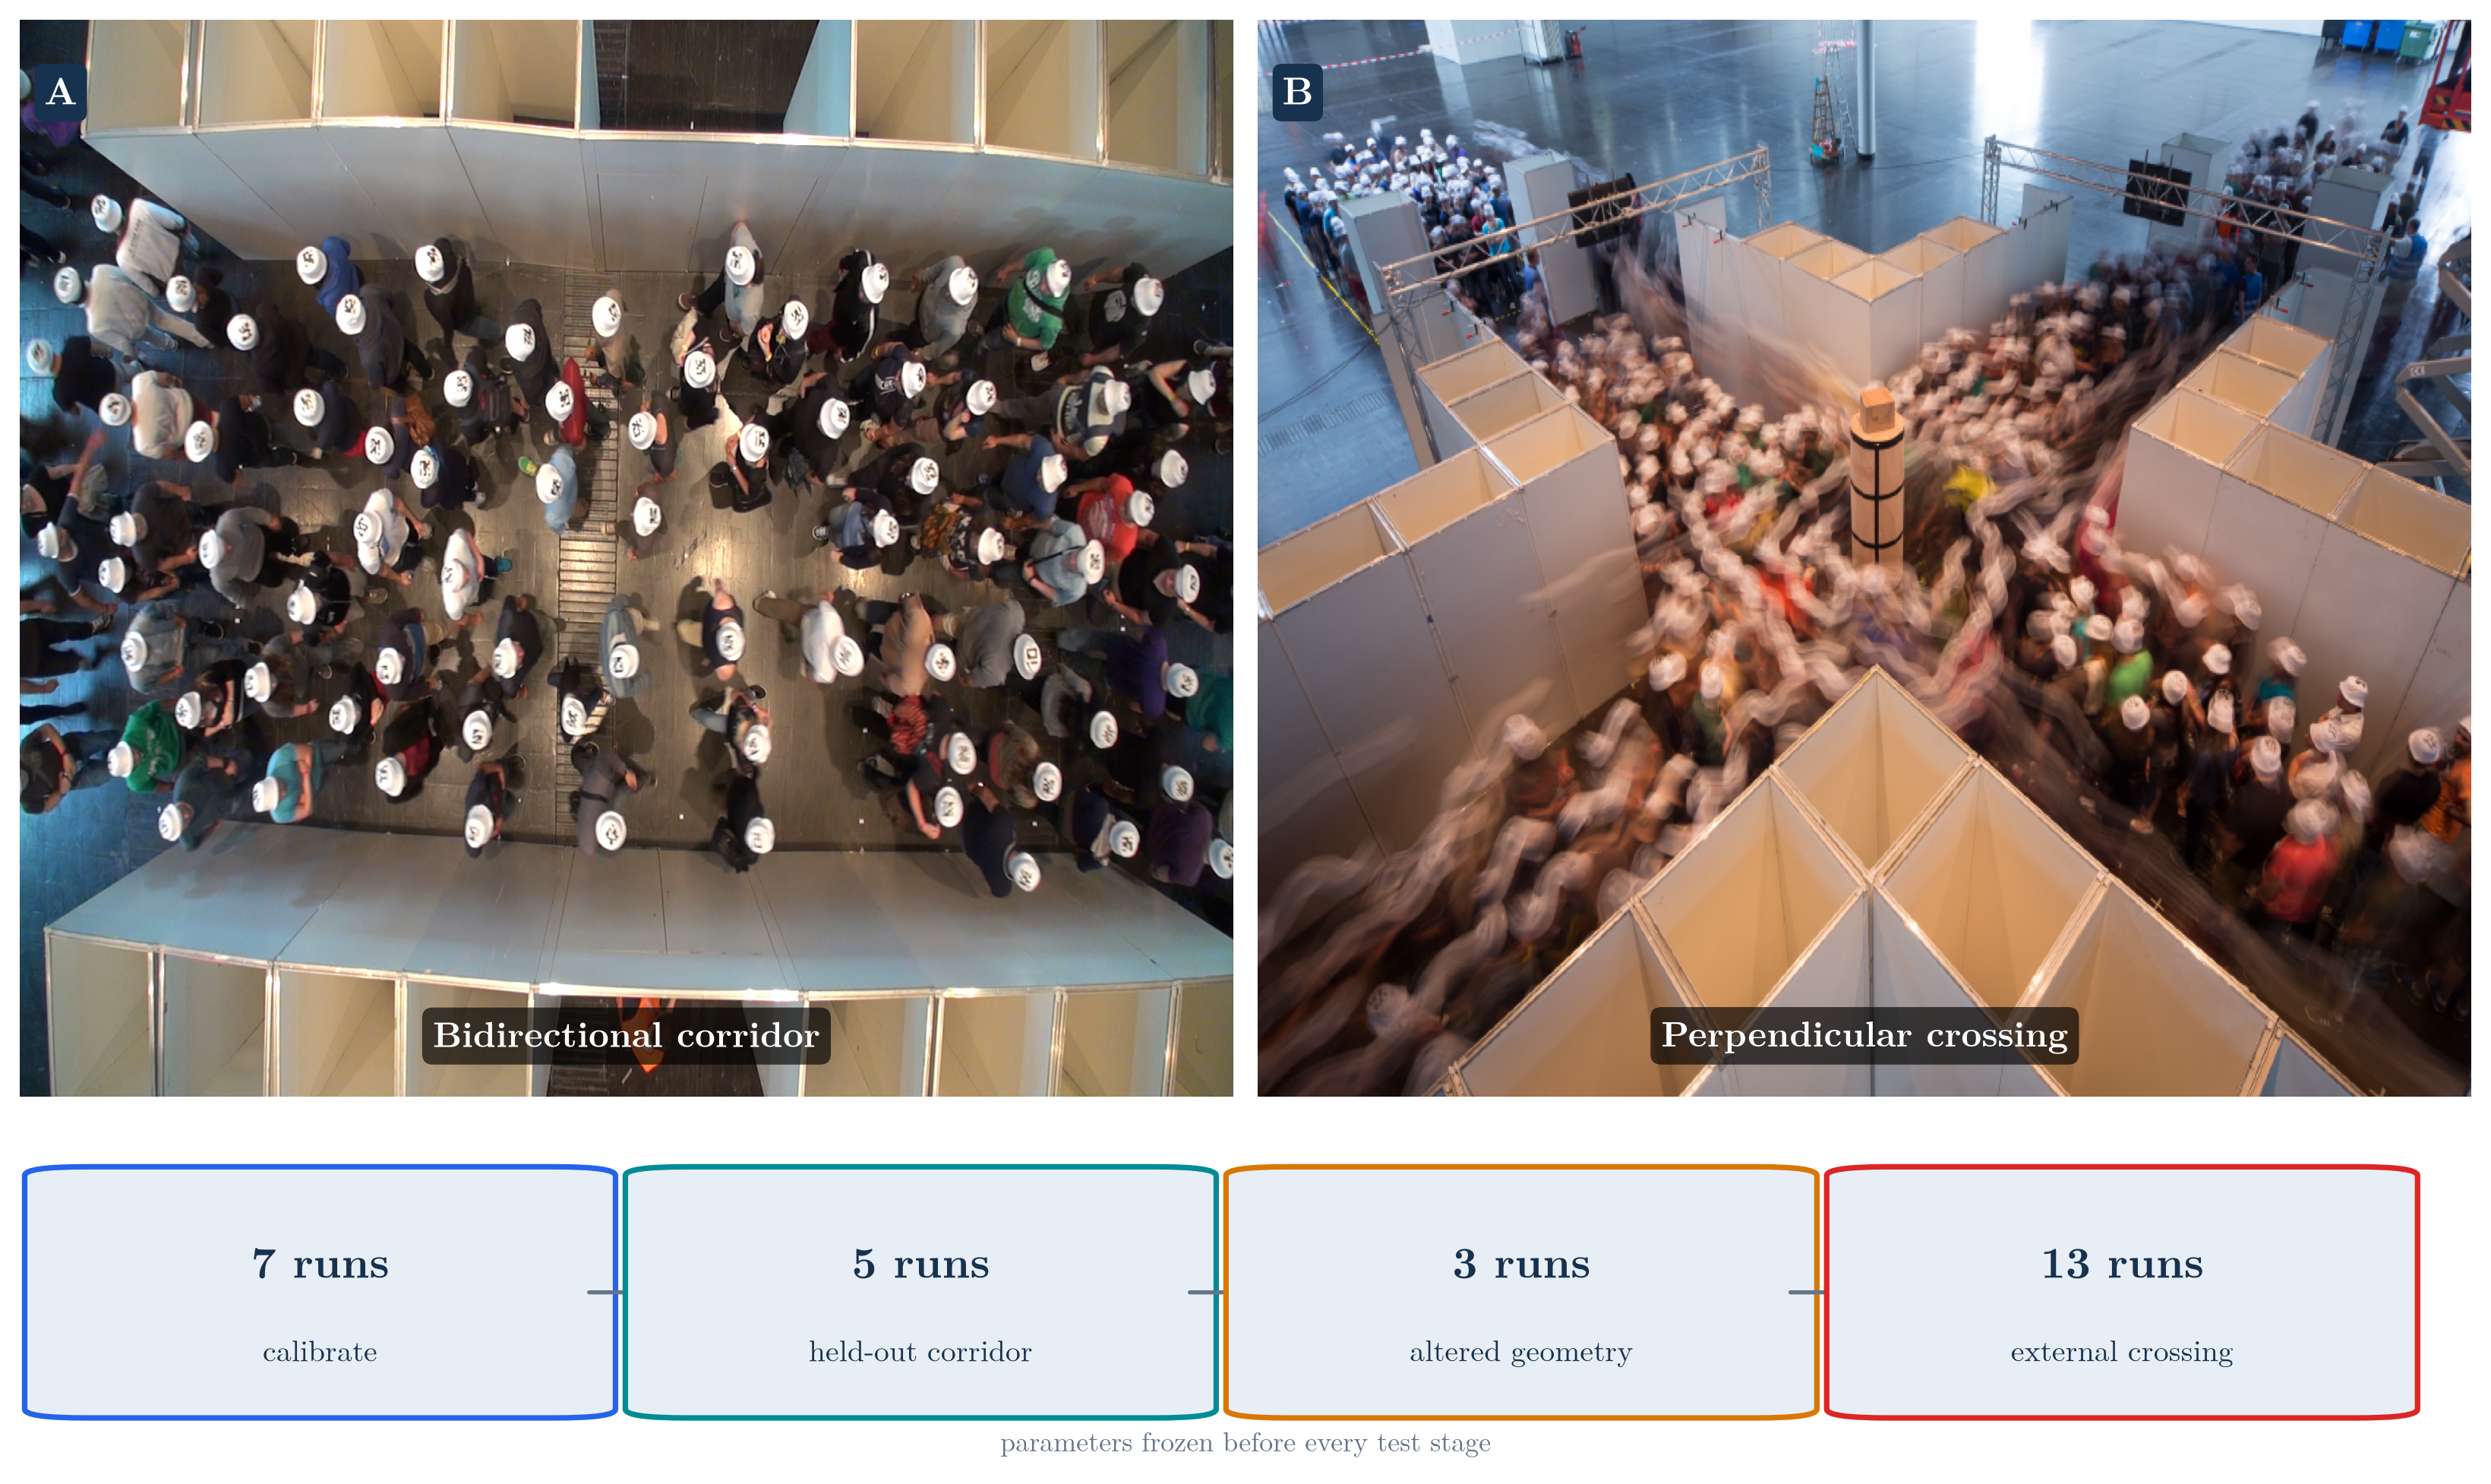
\includegraphics[width=0.98\textwidth]{figures/experimental_context_and_protocol.png}
\caption{Real experiments and frozen evaluation protocol. Overhead views show the corridor and crossing facilities. Seven complete runs calibrate the models; five familiar corridor runs, three altered-geometry runs, and thirteen perpendicular-crossing runs remain untouched. Images: Juelich Pedestrian Dynamics Data Archive, CC BY 4.0; DOIs 10.34735/ped.2013.5 and 10.34735/ped.2013.4.}
\label{fig:1}
\end{figure}

\section{Related work and the unresolved comparison}

\subsection{Operational pedestrian dynamics}

The Social Force Model represents pedestrian motion as relaxation toward a desired velocity plus pedestrian and boundary interactions \citep{helbing1995}. Later specifications introduced angular sensitivity and relative-motion effects, making the response explicitly anisotropic \citep{johansson2007}. Anticipatory models describe collision avoidance through predicted conflicts or time to collision \citep{zanlungo2011,karamouzas2014}, while visually motivated heuristics model navigation as an integrated directional decision \citep{moussaid2011}. Force-based formulations remain useful operational references because their terms are observable, but calibration and the distinction between behavioural and physical acceleration require care \citep{chraibi2011}.

Velocity-space and navigation-field approaches offer related alternatives. Reciprocal velocity obstacles select mutually collision-avoiding velocities \citep{vandenberg2008}. The Anticipation Velocity Model combines direction selection with a collision-free speed rule and reproduces several collective patterns \citep{xu2021}. Continuum and gradient approaches represent route cost or travel time directly \citep{hughes2002,hartmann2010,dietrich2014}. These studies establish that directional response, geometry, and anticipation are not new in isolation. The question here is whether a deliberately small directional prior improves a matched neural forecaster under restricted calibration and unseen topology.

\subsection{Neural and hybrid prediction}

Sequence and interaction models such as Social-LSTM, Social-GAN, Social-STGCNN, and Trajectron++ learn social context from observed trajectories \citep{alahi2016,gupta2018,mohamed2020,salzmann2020}. More recent architectures use graphs, attention, environmental context, multimodal outputs, and intent cues. \citet{su2024} unify social and environmental context in a polar representation, and \citet{munir2025} couple intent and trajectory prediction using local and global scene information. These models target longer, often multimodal trajectories and may use imagery or richer histories. Their published numbers cannot be inserted into a short-horizon dense-crowd table without changing the information and target.

Hybrid models seek the regularization or credibility of structure without discarding learning, but their priors address different failure modes. \citet{wang2024dynamics} embed an asymptotically stable goal-directed dynamical system in a Transformer. \citet{liu2024} extract and aggregate interpretable interaction modes. \citet{pouw2024} infer effective motion laws from laboratory and station data, \citet{sang2024} impose neural differential constraints, \citet{mai2025} update interpretable route and speed modules online, and \citet{xu2026} combine learned pushing states with physics-based movement strategies. None of these contributions is diminished by the present work. They instead expose the missing comparison: goal convergence, generic physical consistency, and interpretability do not establish whether explicitly decoupling progress and lateral avoidance reduces site-specific estimation demand or loss under a new interaction topology.

\subsection{From literature gap to contribution}

Published sequence and hybrid models establish performance in their native protocols, but their reported numbers cannot isolate the value of GEL-Ped's directional prior because history, endpoints, imagery, horizons, and sampling differ. The benchmark therefore uses matched information rather than importing incompatible leaderboard scores. An unconstrained network tests whether the prior adds value beyond neural capacity, while a one-step goal-stable hybrid implements the defining stability constraint of \citet{wang2024dynamics} without future-endpoint access. Calibrated Social Force supplies an operational reference, and unrestricted linear regression tests whether any gain is merely a rearrangement of the same projected features. Together these comparators isolate the paper's specific question: whether separating longitudinal progress from lateral avoidance improves estimation and frozen topology transfer.

This positioning leads to three testable expectations. First, a direct network should be difficult to beat when calibration and evaluation share a corridor topology. Second, if the directional prior improves transfer rather than merely one tuned target, its crossing advantage should persist across forecast horizons and against the goal-stable hybrid. Third, under a fixed model design, its estimation advantage should grow as site-specific fitting runs are removed. The experiments are organized around these expectations rather than a broad leaderboard assembled from incompatible datasets.

\section{GEL-Ped method}

\subsection{Prediction task and design rationale}

At observation time $t$, pedestrian $i$ has position $\mathbf{x}_i(t)$, an observed past displacement, a route direction, neighbouring positions and velocities, and available boundary geometry. The task is to predict average velocity over a future horizon $\Delta$. The prior velocity is

\begin{equation}
\label{eq:1}
\begin{split}
\mathbf{v}_i^{-}(t)=\frac{\mathbf{x}_i(t)-\mathbf{x}_i(t-\Delta)}{\Delta}.\\
\end{split}
\end{equation}

The specification follows three behavioural requirements. Persistence is included because short-horizon motion is strongly inertial even when the model is not a physical acceleration law. Goal progress and lateral motion are separated because slowing, advancing, and sidestepping have different operational meanings. Neighbour effects are represented by distance, whether a neighbour is ahead, and whether the pair is closing; wall effects are lateral because the tested boundaries constrain cross-route motion. These components are intentionally few, observable from trajectories, and shared by both neural experts.

Let $\mathbf{e}_i$ be the unit route direction and $\boldsymbol{\ell}_i=(-e_{iy},e_{ix})$ its left-normal unit vector. The primary route estimate is obtained from early observed motion and never from the future endpoint. The pair $(\mathbf{e}_i,\boldsymbol{\ell}_i)$ defines a local frame in which the first output component is route progress and the second is lateral correction.

\subsection{Observed interaction fields}

For a neighbour $j$, define separation $d_{ij}$, the unit vector $\mathbf{u}_{ij}$ pointing from $i$ to $j$, the away vector $\mathbf{n}_{ij}=-\mathbf{u}_{ij}$, and the observed rate of separation $\dot d_{ij}$:

\begin{equation}
\label{eq:2}
d_{ij}=\lVert\mathbf{x}_j-\mathbf{x}_i\rVert,\quad \mathbf{u}_{ij}=\frac{\mathbf{x}_j-\mathbf{x}_i}{d_{ij}},\quad \dot d_{ij}=(\mathbf{v}_j^{\mathrm{obs}}-\mathbf{v}_i^{\mathrm{obs}})^{\mathsf T}\mathbf{u}_{ij}.
\end{equation}

An exponential proximity weight $q_{ij}$ is truncated beyond a neighbour cutoff. Three pedestrian fields then summarize different aspects of the local interaction:

\begin{equation}
\label{eq:3}
q_{ij}=\exp[-(d_{ij}-2R)/B],\quad \mathbf{r}_i^{\mathrm{iso}}=\sum_j q_{ij}\mathbf{n}_{ij}.
\end{equation}

\begin{equation}
\label{eq:4}
\mathbf{r}_i^{\mathrm{front}}=\sum_j q_{ij}\max(\mathbf{e}_i^{\mathsf T}\mathbf{u}_{ij},0)^2\mathbf{n}_{ij},\quad \mathbf{r}_i^{\mathrm{close}}=\sum_j q_{ij}\max(-\dot d_{ij},0)\mathbf{n}_{ij}.
\end{equation}

The isotropic field summarizes surrounding pressure, the forward field emphasizes neighbours in the intended direction, and the closing field emphasizes approaching pairs. For boundary segment $w$, with inward unit normal $\mathbf{n}_{iw}$ and perpendicular distance $d_{iw}$, the wall field is

\begin{equation}
\label{eq:5}
\mathbf{r}_i^{\mathrm{wall}}=\sum_w \exp(-d_{iw}/B_w)\mathbf{n}_{iw}.
\end{equation}

Together with persistence $\mathbf{v}_i^{-}$ and goal $\mathbf{e}_i$, these fields form the common observed state. Numerical ranges, cutoffs, and sampling choices are deliberately deferred to the experimental design section.

\subsection{Tensor-response prior}

For field $k$, the response tensor is diagonal in the pedestrian frame:

\begin{equation}
\label{eq:6}
\mathbf{T}_i^{(k)}=\beta_{\parallel k}\mathbf{e}_i\mathbf{e}_i^{\mathsf T}+\beta_{\perp k}\boldsymbol{\ell}_i\boldsymbol{\ell}_i^{\mathsf T}.
\end{equation}

The tensor prior combines the projected fields as

\begin{equation}
\label{eq:7}
\widehat{\mathbf{v}}_i^{T}=\sum_k\mathbf{T}_i^{(k)}\mathbf{r}_i^{(k)}=(\boldsymbol{\beta}_{\parallel}^{\mathsf T}\mathbf{z}_i^{\parallel})\mathbf{e}_i+(\boldsymbol{\beta}_{\perp}^{\mathsf T}\mathbf{z}_i^{\perp})\boldsymbol{\ell}_i.
\end{equation}

The longitudinal channel uses persistence, goal, isotropic, forward, and closing projections. The lateral channel uses persistence, isotropic, forward, closing, and wall projections. Goal is excluded laterally because it defines progress rather than avoidance; wall response is excluded longitudinally because the corridor walls do not provide a route-progress cue. This gives ten fitted coefficients. The restrictions encode the proposed behavioural claim, while an unrestricted linear baseline later tests whether those restrictions are useful.

\subsection{Structured residual expert}

A linear tensor cannot represent every local response. The structured expert therefore predicts the residual left after the tensor prior. Let $\boldsymbol{\phi}_i$ contain all common vector fields projected onto the local frame together with the tensor prediction. A multilayer perceptron $G_{\psi}$ predicts a two-component local residual. Its contribution is reduced when the design point lies outside calibration support:

\begin{equation}
\label{eq:8}
s_i=\sqrt{p^{-1}\lVert\operatorname{standardize}(\boldsymbol{\phi}_i)\rVert^2},\quad g_i=\left[1+\gamma\max(s_i/s_q-1,0)^2\right]^{-1}.
\end{equation}

Here $s_q$ is a calibration-only quantile of the support score and $\gamma$ controls smooth shrinkage. The structured expert is

\begin{equation}
\label{eq:9}
\widehat{\mathbf{v}}_i^{S}=\widehat{\mathbf{v}}_i^{T}+g_i\left(G_{\psi,\parallel}(\boldsymbol{\phi}_i)\mathbf{e}_i+G_{\psi,\perp}(\boldsymbol{\phi}_i)\boldsymbol{\ell}_i\right).
\end{equation}

This construction makes the prior consequential: the network learns only what the tensor leaves unexplained, and its correction becomes conservative as calibration support weakens. The gate is not a hidden confidence claim; it is recorded for every forecast and examined empirically.

\subsection{Direct neural expert and calibrated blend}

The direct expert $F_{\theta}$ uses the same standardized local fields and the same hidden-layer architecture but predicts future local velocity directly:

\begin{equation}
\label{eq:10}
\widehat{\mathbf{v}}_i^{N}=F_{\theta,\parallel}(\boldsymbol{\phi}_i^{N})\mathbf{e}_i+F_{\theta,\perp}(\boldsymbol{\phi}_i^{N})\boldsymbol{\ell}_i.
\end{equation}

The final forecast is a convex combination

\begin{equation}
\label{eq:11}
\widehat{\mathbf{v}}_i=\lambda\widehat{\mathbf{v}}_i^{N}+(1-\lambda)\widehat{\mathbf{v}}_i^{S},\quad 0\leq\lambda\leq1.
\end{equation}

The blend allows the model to retain neural interpolation skill while using a differently regularized expert. Crucially, $\lambda$ is selected on calibration runs only. The external crossing data cannot decide whether the structured expert or the blend is reported.

\hyperref[fig:2]{Figure~\ref*{fig:2}} summarizes GEL-Ped and the information flow between its two experts.

\begin{figure}[!htbp]
\centering
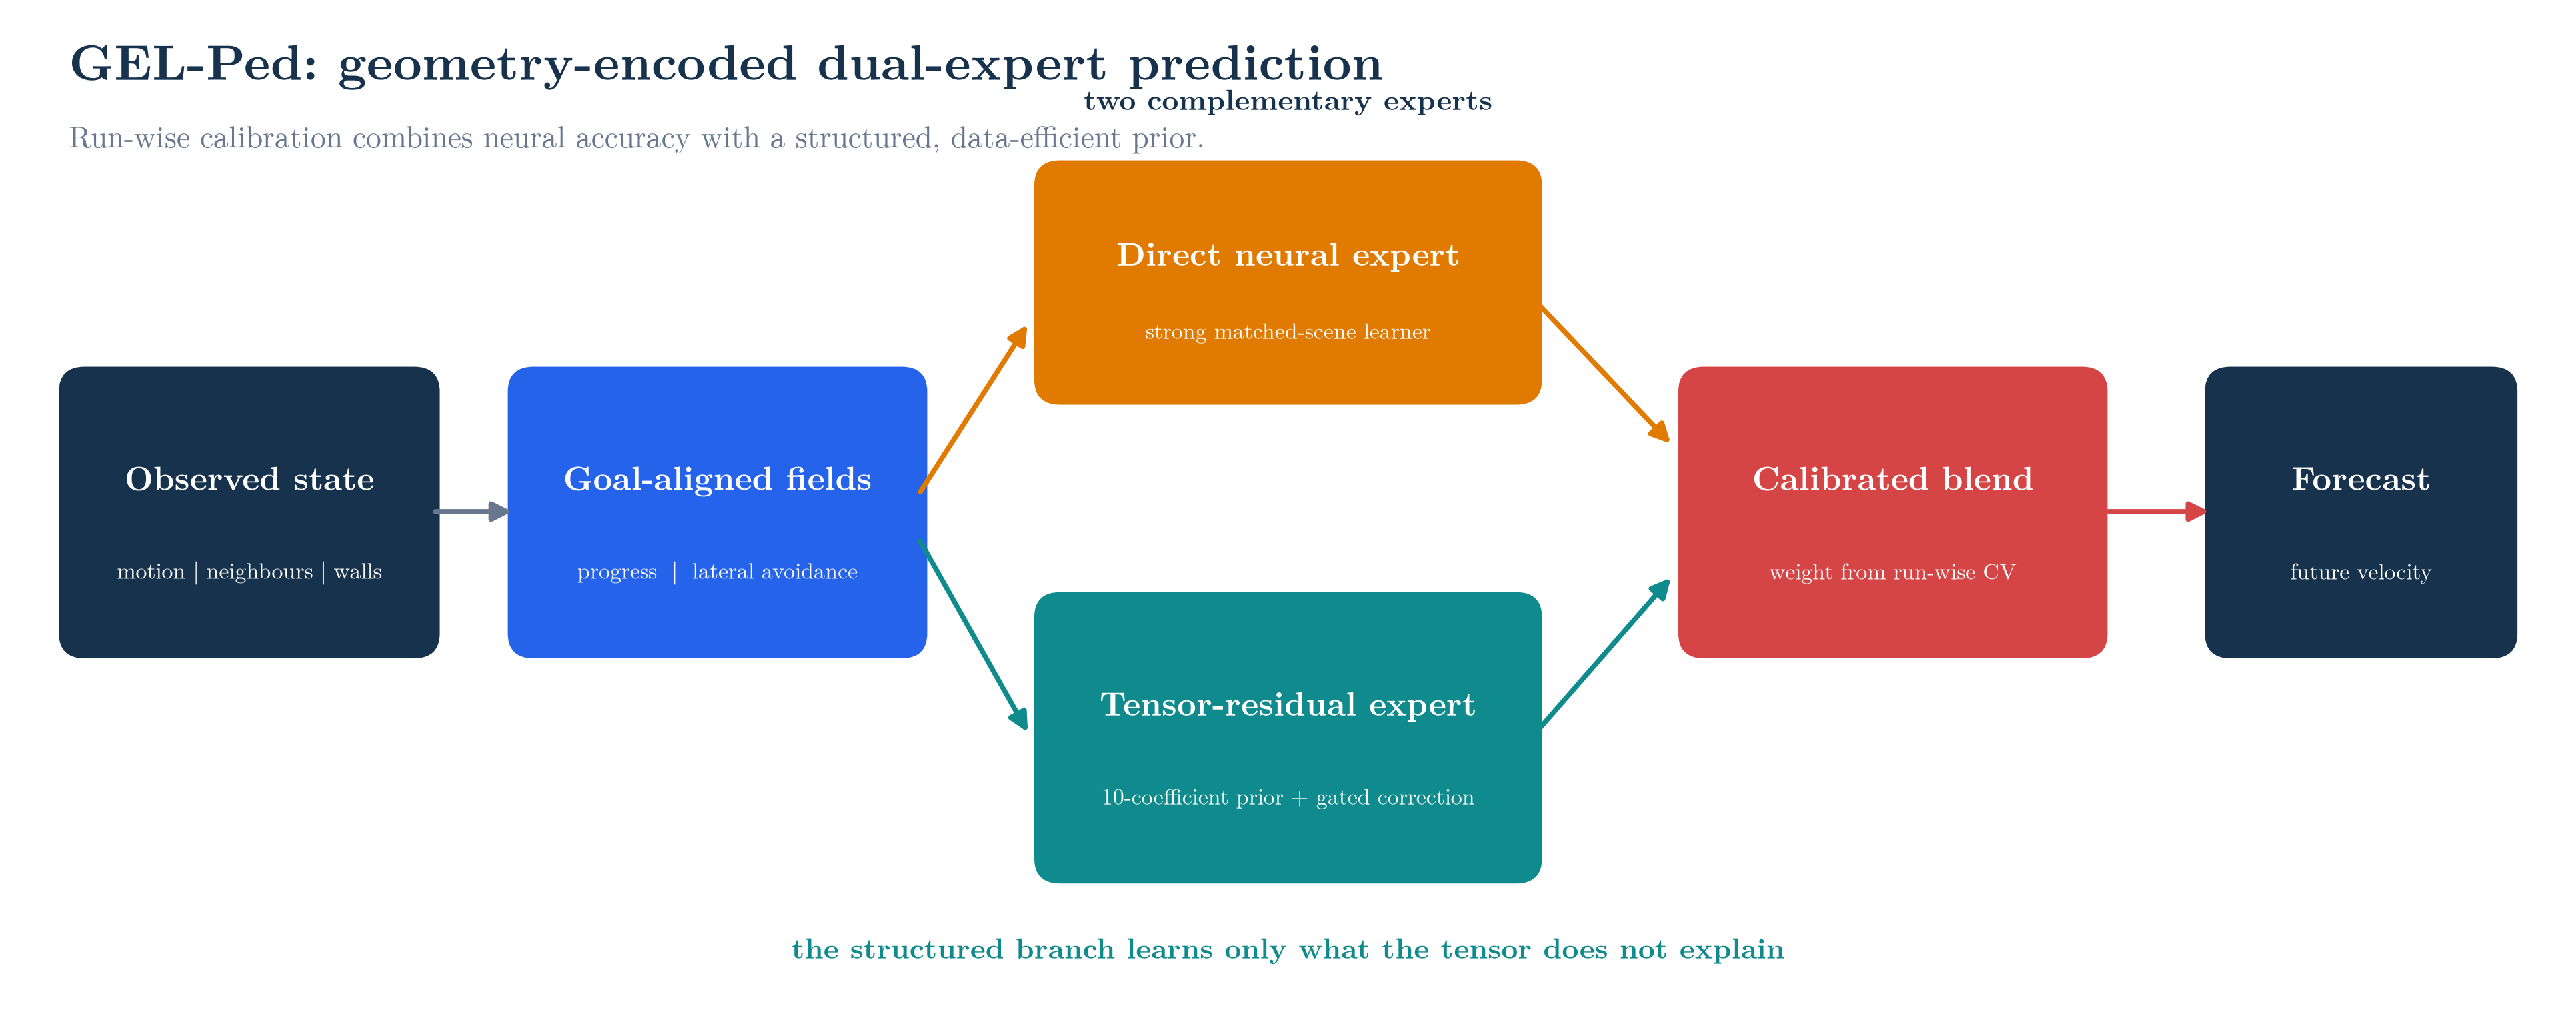
\includegraphics[width=0.95\textwidth]{figures/tensor_residual_architecture.png}
\caption{GEL-Ped dual-expert architecture. A direct neural expert learns the full mapping in the goal-aligned frame. A structured expert starts from the tensor response and learns a support-gated nonlinear residual. A run-wise calibrated convex blend combines their complementary predictions.}
\label{fig:2}
\end{figure}

\subsection{Notation and equivariance}

\hyperref[tab:1]{Table~1} defines the symbols used in the GEL-Ped specification and separates fitted quantities from observed inputs.

\begin{table}[!htbp]
\centering
\caption{Notation used in GEL-Ped.}
\label{tab:1}
\small
\renewcommand{\arraystretch}{1.13}
\setlength{\tabcolsep}{5pt}
\begin{tabularx}{\textwidth}{>{\raggedright\arraybackslash}p{0.20\textwidth}*{3}{>{\raggedright\arraybackslash}X}}
\toprule
Symbol & Meaning & Type or unit & Role in the model \\
\midrule
$\mathbf{x}_i(t)$ & Position of pedestrian $i$ & Vector, m & Observed state \\
$\mathbf{v}_i^{-}$ & Past average velocity & Vector, m/s & Persistence field \\
$\mathbf{e}_i,\boldsymbol{\ell}_i$ & Route and lateral unit directions & Unit vectors & Local pedestrian frame \\
$d_{ij},\dot d_{ij}$ & Pair distance and separation rate & m, m/s & Proximity and closing response \\
$R,B,B_w,D$ & Body radius, interaction range, wall range, neighbour cutoff & m & Field scales \\
$\mathbf{r}^{\mathrm{iso}},\mathbf{r}^{\mathrm{front}},\mathbf{r}^{\mathrm{close}},\mathbf{r}^{\mathrm{wall}}$ & Observed interaction fields & Vectors & Common inputs to both experts \\
$\mathbf{T}^{(k)}$ & Direction-specific response tensor for field $k$ & Rank-two tensor & Structured linear prior \\
$\boldsymbol{\beta}_{\parallel},\boldsymbol{\beta}_{\perp}$ & Longitudinal and lateral coefficients & Mixed units & Fitted tensor response \\
$G_{\psi},F_{\theta}$ & Residual and direct neural mappings & Functions & Structured and direct experts \\
$s_i,s_q,g_i$ & Support score, threshold, and gate & Dimensionless & Shrink residual outside support \\
$\lambda$ & Direct-expert blend weight & Dimensionless & Calibration-selected GEL-Ped blend \\
$\Delta$ & Forecast horizon & s & Prediction interval \\
\bottomrule
\end{tabularx}
\end{table}

If the route and every observed vector are rotated by $\mathbf{Q}\in SO(2)$, then $\mathbf{T}'=\mathbf{Q}\mathbf{T}\mathbf{Q}^{\mathsf T}$ and each local scalar projection is unchanged. Both neural networks operate on those invariant scalar projections, and recombination uses the rotated basis. Therefore $\widehat{\mathbf{v}}'=\mathbf{Q}\widehat{\mathbf{v}}$. The model head is rotation-equivariant for a covariant route input. The primary route estimator uses cardinal entry directions from the controlled facilities, so the complete pipeline is guaranteed only for rotations that preserve those classes, including the tested right-angle change.

\section{Experimental design}

\subsection{Data, real-world context, and frozen partitions}

The first dataset is the open Juelich bidirectional-corridor archive (DOI 10.34735/ped.2013.5). Participants walked through controlled corridor configurations and trajectories were extracted from overhead video using PeTrack \citep{boltes2013,boltes2020}. Seven complete runs calibrate every model and selection decision. Five standard-geometry runs are untouched familiar-corridor tests. Three further runs with changed corridor length or exit arrangement form the altered-geometry test.

The external dataset is the open BaSiGo right-angle crossing archive (DOI 10.34735/ped.2013.4). All thirteen available part D and E runs are used as an external test. They contain two streams approaching at right angles and are never used to fit a coefficient, neural weight, support threshold, epoch count, architecture, or blend. The wall input is set to zero because a matching two-wall corridor representation is absent; every learned quantity remains frozen.

The primary route direction is the dominant cardinal displacement during the first observation horizon of each trajectory. Forecasts begin only after that history exists. Endpoint direction is never used in the main analysis. The test sets contain 28,507 familiar-corridor forecasts, 18,000 altered-geometry forecasts, and 78,000 crossing forecasts.

\hyperref[fig:1]{Figure~\ref*{fig:1}}'s protocol separates development from evidence. The unit of independence is the complete experimental run, not an individual pedestrian-frame pair.

\subsection{Sampling, calibration, and numerical settings}

\hyperref[tab:2]{Table~2} reports all numerical choices in one place. Fixed geometric values follow the controlled-experiment scale and conventional interpersonal-distance ranges; sensitivity checks vary the interaction range and neighbour cutoff. Neural architecture, epoch count, residual epoch count, speed cap, ridge penalty, support threshold, and blend weight are selected by leave-one-calibration-run-out validation. The inactive speed cap means no reported gain is created by clipping predictions.

\begin{table}[!htbp]
\centering
\caption{Numerical settings, calibration results, and their justification.}
\label{tab:2}
\small
\renewcommand{\arraystretch}{1.13}
\setlength{\tabcolsep}{5pt}
\begin{tabularx}{\textwidth}{>{\raggedright\arraybackslash}p{0.20\textwidth}*{3}{>{\raggedright\arraybackslash}X}}
\toprule
Group & Setting & Value & Justification or selection rule \\
\midrule
Sampling & Frame rate; horizon; stride & 25 Hz; 10 frames (0.4 s); 10 frames & Native archive rate; non-overlapping target windows \\
Sampling & Maximum forecasts per run; seed & 6,000; 20260722 & Prevent a long run dominating; reproducibility \\
Data quality & Observed-speed exclusion & Above 3.0 m/s & Remove tracking outliers, not model predictions \\
Interaction & $R;B;B_w;D$ & 0.25; 0.80; 0.25; 3.0 m & Body scale, local decay, wall decay, and finite neighbourhood \\
Tensor fit & Coefficient bounds & [-5, 5] & Broad signed bounds; no estimate approaches a bound \\
Neural experts & Hidden layers; activation; batch & 64--64; tanh; 256 & Best of three run-wise candidates with matched expert capacity \\
Direct expert & L2 penalty; epochs & 0.01; 40 & Complete-run cross-validation and run-level early stopping \\
Residual expert & L2 penalty; epochs & 0.01; 120 & Complete-run residual-epoch search over 20, 40, 80, 120 \\
Support gate & Quantile $q$; strength $\gamma$ & 0.95; 4.0 & Calibration-only support boundary and smooth shrinkage \\
GEL-Ped & Direct weight $\lambda$ & 0.50 & Minimum mean calibration-run CV RMSE over 0, 0.25, 0.50, 0.75, 1 \\
Prediction & Selected speed cap & 100 m/s & Operationally inactive; selected from 2, 2.5, 3, 100 m/s \\
Social Force fit & Relaxation time; desired speed & 3.295 s; 0.694 m/s & Run-balanced nonlinear least squares within broad physical bounds \\
Social Force fit & Pedestrian; wall acceleration scale & 0.0166; 0.4488 m/s\textsuperscript{2} & Run-balanced calibration of exponential-distance fields \\
Uncertainty & Run bootstrap; hierarchical bootstrap & 20,000; 2,000 draws & Run-level intervals and within-run sensitivity \\
\bottomrule
\end{tabularx}
\end{table}

The interaction range is varied from 0.2 to 1.6 m and the neighbour cutoff from 2 to 4 m on calibration folds. The resulting calibration RMSE range is small, so the selected scales are treated as stable working values rather than uniquely identified behavioural constants. Five neural seeds are evaluated after the primary seed is frozen.

\subsection{Focused and fair reference models}

Five comparators are predeclared for confirmatory tests. \textbf{Constant velocity} has no fitted parameters and measures the value beyond short-horizon persistence. \textbf{Calibrated Social Force} is an observed-state discretization of the established desired-motion plus exponential pedestrian and wall response \citep{helbing1995,johansson2007}:

\begin{equation}
\label{eq:12}
\widehat{\mathbf{v}}_i^{SF}=\mathbf{v}_i^{-}+\Delta\left[\frac{v_0\mathbf{e}_i-\mathbf{v}_i^{-}}{\tau}+a_p\mathbf{r}_i^{\mathrm{iso}}+a_w\mathbf{r}_i^{\mathrm{wall}}\right].
\end{equation}

Its four parameters are fitted with the same run-balanced objective. \textbf{Unrestricted linear} predicts both local output components from all ten tensor projections, with two intercepts and no proposed zero restrictions; it directly tests whether the tensor specification adds value beyond an equally informed linear mapping. \textbf{Direct neural} is the decisive capacity control: it receives the same projected observed fields as GEL-Ped, uses the same 64--64 architecture as each neural branch, and predicts the target without a tensor prior.

\textbf{Goal-stable neural} supplies a recent hybrid reference derived from the dynamics-based deep-learning model of \citet{wang2024dynamics}. Their published system combines a Transformer, goal estimator, and positive-definite goal-directed dynamics over a longer trajectory protocol. Importing its published scores or future-endpoint training would be unfair here. We instead implement its defining one-step constraint under exactly the present observations: positive-definite attraction implies non-negative predicted progress along the observed route, so the matched direct-network output is projected onto that feasible half-space while retaining its lateral prediction. This is the least-squares one-step realization of the stability constraint, uses the same 5,122 neural parameters, and never accesses a future endpoint. It is explicitly a protocol-matched hybrid reference rather than a claim to reproduce the authors' long-horizon Transformer leaderboard.

Additional models are used only as ablations: the ten-coefficient tensor prior, the tensor plus gated residual, and the same residual without its support gate. Long-history multimodal models are not inserted as numerical baselines because doing so would change input history, target distribution, scene imagery, and often prediction horizon. Their role is literature positioning; the direct and goal-stable neural references isolate unconstrained capacity and an alternative hybrid prior under the current task.

\subsection{Metrics and inference}

For run $r$, the primary metric is vector velocity RMSE,

\begin{equation}
\label{eq:13}
\mathrm{RMSE}_{v,r}=\sqrt{N_r^{-1}\sum_{n=1}^{N_r}\lVert\widehat{\mathbf{v}}_{nr}-\mathbf{v}_{nr}\rVert^2}.
\end{equation}

Headline values are arithmetic means of run-specific metrics, so every experiment has equal weight. Secondary outcomes are displacement MAE over the prediction horizon, speed MAE, median heading error, vector (R\textasciicircum{}2), and false short-horizon contacts. A false contact occurs when a pair initially within the evaluation neighbourhood is predicted to finish closer than 0.4 m although its observed final separation is at least 0.4 m. This is a plausibility diagnostic, not a collision-avoidance guarantee \citep{korbmacher2024}.

Paired differences use an exact sign-flip randomization test. Ninety-five percent intervals are obtained by resampling complete runs; a hierarchical sensitivity additionally resamples paired forecasts within each selected run. The five confirmatory comparators are adjusted with Holm's procedure within each reported test regime. The cross-horizon neural comparison uses 0.2, 0.4, 0.8, and 1.2 s targets with non-overlapping forecast windows and settings frozen from the primary analysis; its four p-values are additionally Holm-adjusted across horizons. Counts of improved runs and exact sign tests are retained so that a small mean is not mistaken for consistent improvement.

The data-efficiency analysis has a narrower interpretation. The architecture and regularization are fixed once by the seven-run development phase; then both models are refitted using every possible subset of those runs. All 127 combinations across one to seven runs are enumerated. This estimates site-specific fitting efficiency for a predesigned model. Because subsets overlap and share the same untouched evaluation runs, their intervals describe robustness to calibration choice rather than 127 independent experiments, and the curve is not used to claim that the architecture itself can be selected from one run. \hyperref[app:A]{Appendix~A} lists the frozen run partitions and the reproducibility map. \hyperref[app:B]{Appendix~B} contains the detailed inferential evidence: \hyperref[tab:B1]{Table~B.1} provides the complete confirmatory comparisons, while \hyperref[tab:B2]{Table~B.2} reports the cross-horizon statistics.

\section{Results}

\subsection{Primary performance and the neural comparison}

\hyperref[tab:3]{Table~3} answers the primary 0.4 s model-choice question. The direct neural model has the lowest error in the familiar corridor and altered-geometry sets. GEL-Ped is 1.03\% worse in the familiar corridor and 0.49\% worse under altered corridor geometry. The goal-stable hybrid is also close to the direct model in both cases. These results prevent a blanket claim that either kind of structure always improves interpolation.

The ordering changes in perpendicular crossing. GEL-Ped reaches 0.3588 m/s compared with 0.3638 m/s for the direct network and 0.3642 m/s for the goal-stable hybrid. Relative reductions are 1.38\% and 1.49\%, respectively, and GEL-Ped is lower than both in eleven of thirteen runs. The run-bootstrap intervals for GEL-Ped minus comparator are [-0.0090, -0.0017] m/s against the direct network and [-0.0094, -0.0021] m/s against the goal-stable hybrid. Exact paired p-values are 0.0117 and 0.0083; Holm-adjusted values across the five confirmatory comparators are 0.0234 and 0.0249. Goal convergence alone therefore does not explain the crossing advantage.

\begin{table}[!htbp]
\centering
\caption{Run-balanced short-horizon performance on untouched experimental runs.}
\label{tab:3}
\footnotesize
\renewcommand{\arraystretch}{1.10}
\setlength{\tabcolsep}{4pt}
\resizebox{\textwidth}{!}{%
\begin{tabular}{lccccc}
\toprule
Test regime & Model & Velocity RMSE (m/s) & Displacement MAE (m) & Median angle (degrees) & False-contact rate \\
\midrule
Familiar corridor (5 runs) & Constant velocity & 0.2315 & 0.0806 & 18.47 & 0.00787 \\
Familiar corridor (5 runs) & Calibrated Social Force & 0.2246 & 0.0787 & 17.21 & 0.00697 \\
Familiar corridor (5 runs) & Unrestricted linear & 0.2106 & 0.0713 & 14.93 & 0.00557 \\
Familiar corridor (5 runs) & \textbf{Direct neural} & \textbf{0.1819} & \textbf{0.0616} & \textbf{11.76} & \textbf{0.00472} \\
Familiar corridor (5 runs) & Goal-stable neural hybrid & 0.1822 & 0.0617 & 11.83 & 0.00465 \\
Familiar corridor (5 runs) & GEL-Ped & 0.1838 & 0.0622 & 12.00 & 0.00491 \\
Altered geometry (3 runs) & Constant velocity & 0.2291 & 0.0791 & 25.07 & 0.01029 \\
Altered geometry (3 runs) & Calibrated Social Force & 0.2227 & 0.0775 & 23.34 & 0.00933 \\
Altered geometry (3 runs) & Unrestricted linear & 0.2054 & 0.0699 & 20.48 & 0.00761 \\
Altered geometry (3 runs) & \textbf{Direct neural} & \textbf{0.1798} & \textbf{0.0610} & \textbf{16.15} & \textbf{0.00676} \\
Altered geometry (3 runs) & Goal-stable neural hybrid & 0.1808 & 0.0612 & 16.29 & \textbf{0.00661} \\
Altered geometry (3 runs) & GEL-Ped & 0.1807 & 0.0613 & 16.46 & 0.00680 \\
Perpendicular crossing (13 runs) & Constant velocity & 0.4127 & 0.1428 & 16.36 & 0.01605 \\
Perpendicular crossing (13 runs) & Calibrated Social Force & 0.3991 & 0.1388 & 15.60 & 0.01459 \\
Perpendicular crossing (13 runs) & Unrestricted linear & 0.3703 & 0.1254 & 13.23 & 0.01218 \\
Perpendicular crossing (13 runs) & Direct neural & 0.3638 & 0.1240 & 12.14 & \textbf{0.01061} \\
Perpendicular crossing (13 runs) & Goal-stable neural hybrid & 0.3642 & 0.1240 & \textbf{12.11} & \textbf{0.01059} \\
Perpendicular crossing (13 runs) & \textbf{GEL-Ped} & \textbf{0.3588} & \textbf{0.1222} & \textbf{12.12} & 0.01066 \\
\bottomrule
\end{tabular}
}
\end{table}

\hyperref[fig:3]{Figure~\ref*{fig:3}} reports the primary comparison visually and shows the complete-run distribution behind the means. Across all twenty-one untouched runs, GEL-Ped lowers run-relative RMSE by 15.97\% against constant velocity, 13.28\% against calibrated Social Force, and 6.53\% against unrestricted linear. All twenty-one runs improve over the first two references, and seventeen improve over unrestricted linear. Each comparison is significant after Holm correction (p<0.001). These larger gains establish value beyond operational and linear references even though the pooled neural comparison is much closer.

\begin{figure}[!htbp]
\centering

\includegraphics[width=0.95\textwidth]{figures/primary_performance_summary.png}
\caption{Primary accuracy results. Bars show run-balanced velocity RMSE and standard errors for the three untouched regimes. Run-level dots and bootstrap intervals show the GEL-Ped reductions relative to constant velocity, calibrated Social Force, and the unrestricted linear model.}
\label{fig:3}
\end{figure}

The pooled mean RMSE is 0.2917 m/s for GEL-Ped, 0.2942 m/s for the direct network, and 0.2947 m/s for the goal-stable hybrid. On a run-relative scale GEL-Ped is 0.54\% lower than the direct model, but its 95\% run-bootstrap interval spans zero [-0.17\%, 1.34\% reduction] and the exact p-value is 0.202. The pooled result is therefore reported as no detected overall difference. The substantive evidence is specific to topology transfer and fixed-design estimation, not universal neural dominance.

\subsection{Transfer across forecast horizons}

\hyperref[fig:4]{Figure~\ref*{fig:4}} tests whether the crossing advantage is an accident of the primary horizon. It is not. Relative to the direct network, crossing RMSE falls by 3.55\% at 0.2 s, 1.38\% at 0.4 s, 4.56\% at 0.8 s, and 2.94\% at 1.2 s. GEL-Ped improves all thirteen crossing runs at 0.2, 0.8, and 1.2 s and eleven of thirteen at 0.4 s. Exact paired p-values are 0.000244, 0.0117, 0.000244, and 0.000244; all remain below 0.05 after Holm correction across the four horizons.

\begin{figure}[!htbp]
\centering

\includegraphics[width=0.95\textwidth]{figures/cross_horizon_neural_transfer.png}
\caption{Cross-horizon topology transfer. Left: run-balanced RMSE on thirteen unseen perpendicular-crossing runs for the direct network, a protocol-matched 2024 goal-stable hybrid, and GEL-Ped. Right: complete-run reductions relative to the direct network with run-bootstrap intervals. Model settings are frozen rather than retuned by horizon.}
\label{fig:4}
\end{figure}

The 0.8 s comparison gives the largest mean effect: RMSE decreases from 0.3542 to 0.3373 m/s and displacement MAE from 0.2273 to 0.2167 m. At 1.2 s, displacement MAE decreases from 0.3635 to 0.3512 m. These centimetre-scale mean displacement reductions are more tangible than the 1.8 mm difference at the primary 0.4 s horizon. The goal-stable hybrid tracks the direct network closely throughout, whereas GEL-Ped remains lower on crossing. The evidence therefore concerns transfer of the interaction prior, not merely the addition of any physical constraint.

\subsection{Fixed-design estimation efficiency}

\hyperref[fig:5]{Figure~\ref*{fig:5}} isolates estimation efficiency after the model design has been fixed. With one site-specific fitting run, the direct network has mean pooled held-out RMSE 0.4019 m/s, whereas GEL-Ped reaches 0.3414 m/s. The reduction is 0.0605 m/s or 14.1\%, with a subset-bootstrap interval of 10.5--18.9\%, and GEL-Ped is better for all seven possible singleton choices.

\begin{figure}[!htbp]
\centering

\includegraphics[width=0.95\textwidth]{figures/data_efficiency.png}
\caption{Fixed-design estimation efficiency. Left: pooled held-out RMSE as the number of site-specific fitting runs increases; shading spans all subsets. Right: reduction from the matched direct neural expert for every subset (circles) and the subset mean (diamonds). All 127 subsets of seven runs are enumerated.}
\label{fig:5}
\end{figure}

Every subset is now enumerated rather than selecting five representative combinations. Mean reductions are 7.29\%, 4.60\%, 2.99\%, 2.16\%, 1.48\%, and 0.87\% as the number of fitting runs increases from two to seven. GEL-Ped is lower in all 127 of 127 subsets. Because these subsets overlap and share evaluation runs, this is a robustness pattern rather than 127 independent replications. It shows that, once the architecture is fixed, structured guidance consistently reduces estimation demand; it does not show that the complete architecture-selection process requires only one run.

\begin{table}[!htbp]
\centering
\caption{Pooled untouched-run accuracy as complete calibration runs are added.}
\label{tab:4}
\footnotesize
\renewcommand{\arraystretch}{1.10}
\setlength{\tabcolsep}{4pt}
\resizebox{\textwidth}{!}{%
\begin{tabular}{lcccc}
\toprule
Calibration runs & Direct neural RMSE (m/s) & GEL-Ped RMSE (m/s) & GEL-Ped reduction & Subset configurations improved \\
\midrule
1 & 0.4019 & 0.3414 & 14.1\% & 7/7 \\
2 & 0.3337 & 0.3087 & 7.3\% & 21/21 \\
3 & 0.3163 & 0.3013 & 4.6\% & 35/35 \\
4 & 0.3058 & 0.2965 & 3.0\% & 35/35 \\
5 & 0.3011 & 0.2945 & 2.2\% & 21/21 \\
6 & 0.2979 & 0.2935 & 1.5\% & 7/7 \\
7 & 0.2942 & 0.2917 & 0.9\% & 1/1 \\
\bottomrule
\end{tabular}
}
\end{table}

\subsection{What each component contributes}

The tensor prior alone is substantially more accurate than constant velocity but cannot match either neural approach in the corridor. Adding a residual closes most of that gap. In crossing flow, the gated tensor residual obtains 0.3625 m/s, the direct network 0.3638 m/s, and GEL-Ped 0.3588 m/s. An ungated residual ablation reaches 0.3563 m/s in crossing, the lowest external mean, but it is not promoted to the primary model because choosing it after viewing crossing outcomes would violate the frozen protocol. Calibration-run selection instead chooses the equal blend.

The support gate behaves as intended but is not the sole source of transfer. The mean gate is 0.99 on calibration, 0.98 on held-out corridor, 0.96 under altered geometry, and 0.97 in crossing. The fraction of forecasts receiving any shrinkage rises from 5\% in calibration to 19\% in crossing. This is a moderate, observable response to distribution shift rather than wholesale rejection of the residual network.

\hyperref[fig:6]{Figure~\ref*{fig:6}} examines model components, gate use, tensor coefficients, and seed sensitivity. Across five optimization seeds, crossing RMSE ranges from 0.3558 to 0.3627 m/s for GEL-Ped and from 0.3628 to 0.3751 m/s for the direct network. Their median values are 0.3600 and 0.3702 m/s, respectively. Familiar-corridor seed ranges overlap, which is consistent with the close interpolation result. \hyperref[tab:C1]{Table~C.1} in \hyperref[app:C]{Appendix~C} reports the complete component means behind this diagnostic, followed by the optimization-seed ranges.

\begin{figure}[!htbp]
\centering

\includegraphics[width=0.95\textwidth]{figures/hybrid_diagnostics.png}
\caption{Component, support, coefficient, and seed diagnostics. The direct network dominates matched-corridor interpolation, while the structured and blended predictors retain more of their accuracy under crossing transfer. The support gate is observable and optimization-seed ranges do not reverse the crossing pattern.}
\label{fig:6}
\end{figure}

\subsection{Interpretable response and plausibility}

\hyperref[tab:5]{Table~5} reports the fitted tensor prior. The strongest coefficient is longitudinal persistence (0.912), while lateral persistence is less than half as large (0.420). This is consistent with route progress being retained more strongly than cross-route drift. Positive forward longitudinal response and negative lateral closing response indicate that neighbours ahead and approaching neighbours affect different output channels. All ten coefficient signs are retained across leave-one-calibration-run-out fits, although bootstrap intervals for three small adjusted effects include zero. Correlated fields mean these are conditional predictive coefficients, not independently identified psychological forces.

\begin{table}[!htbp]
\centering
\caption{Tensor-prior coefficients fitted on seven calibration runs.}
\label{tab:5}
\footnotesize
\renewcommand{\arraystretch}{1.10}
\setlength{\tabcolsep}{4pt}
\resizebox{\textwidth}{!}{%
\begin{tabular}{lcccc}
\toprule
Channel & Feature & Estimate & Run-bootstrap 95\% interval & Sign retained in leave-one-run-out fits \\
\midrule
Longitudinal & Persistence & 0.9115 & [0.8747, 0.9231] & 7/7 \\
Longitudinal & Goal & 0.1033 & [0.0898, 0.1365] & 7/7 \\
Longitudinal & Isotropic & -0.00166 & [-0.00343, 0.00020] & 7/7 \\
Longitudinal & Forward & 0.01893 & [0.01581, 0.02912] & 7/7 \\
Longitudinal & Closing & 0.00279 & [-0.00195, 0.00430] & 7/7 \\
Lateral & Persistence & 0.4201 & [0.2575, 0.5314] & 7/7 \\
Lateral & Isotropic & 0.01311 & [0.00736, 0.01976] & 7/7 \\
Lateral & Forward & -0.01843 & [-0.04581, 0.01555] & 7/7 \\
Lateral & Closing & -0.03386 & [-0.05583, -0.01611] & 7/7 \\
Lateral & Wall & 0.05929 & [0.01652, 0.15810] & 7/7 \\
\bottomrule
\end{tabular}
}
\end{table}

False-contact rates tell a compatible but more cautious story. In crossing, GEL-Ped and the direct network are effectively tied at 0.01066 and 0.01061, both below unrestricted linear (0.01218), Social Force (0.01459), and constant velocity (0.01605). GEL-Ped's accuracy improvement over the direct network does not come with a measurable false-contact advantage. It does preserve the direct network's plausibility level while improving crossing velocity and displacement errors.

\hyperref[fig:7]{Figure~\ref*{fig:7}} shows a representative crossing frame. It is selected by a reproducible rule rather than visual preference: among frames with at least twenty pedestrians and a positive GEL-Ped gain, it is closest to the median gain. The aggregate comparison across thirteen runs remains the evidence; the arrows show what a difference of this scale looks like in a crowded scene.

\begin{figure}[!htbp]
\centering
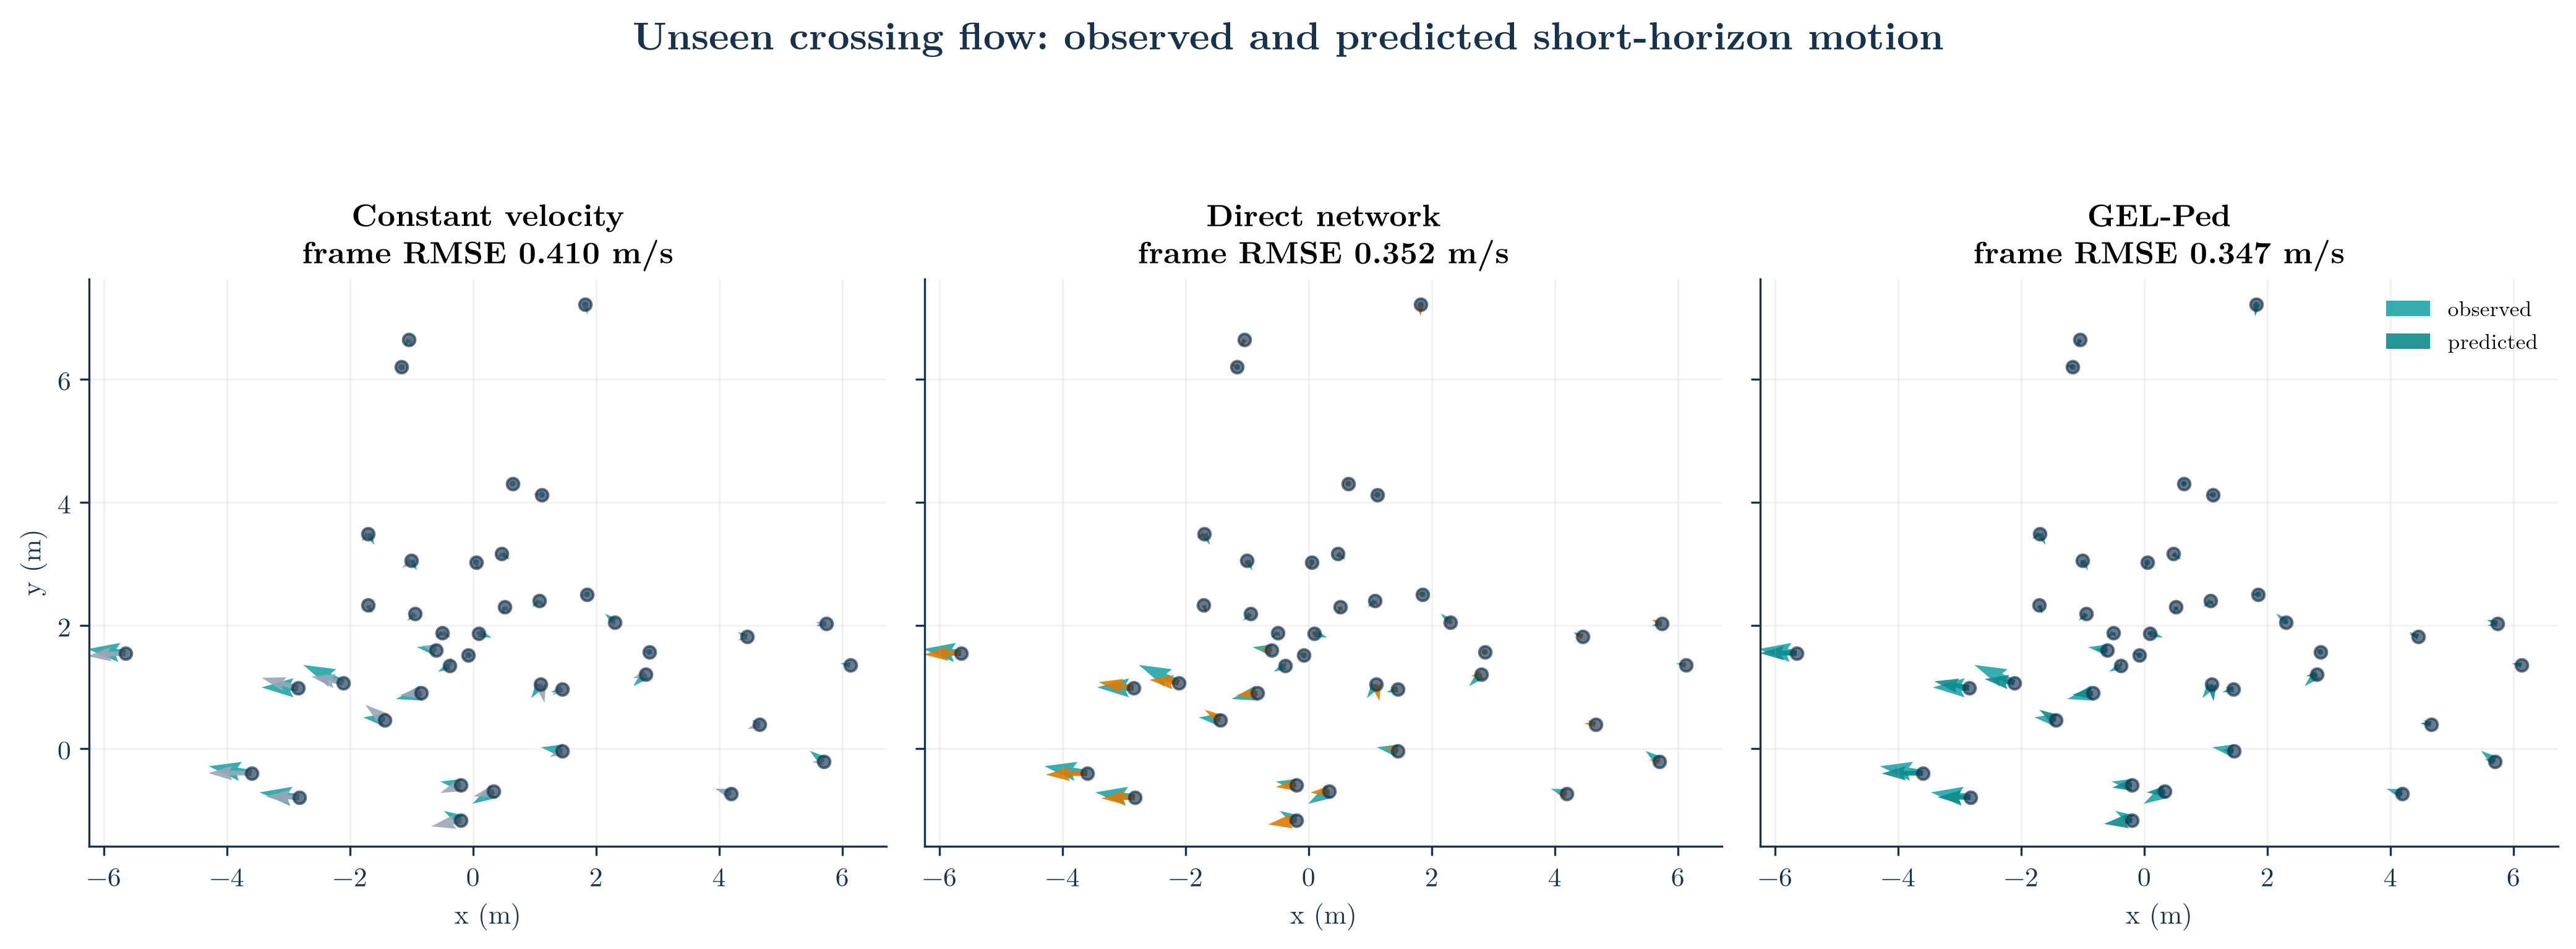
\includegraphics[width=0.95\textwidth]{figures/external_crossing_hybrid_snapshot.png}
\caption{Illustrative unseen-crossing frame. Arrows compare observed future velocity with constant-velocity, direct-network, and GEL-Ped forecasts. The frame is selected reproducibly as the median positive GEL-Ped gain among frames containing at least twenty pedestrians; aggregate run-level tests provide the inferential evidence.}
\label{fig:7}
\end{figure}

\section{Discussion}

\subsection{Why not use the neural model alone?}

For a familiar facility with sufficient representative data, the answer may be: use it. At the primary horizon the direct network is the best model in both corridor regimes, and GEL-Ped should not be justified by interpretability when its prediction is slightly worse. The evidence supports GEL-Ped for a different operating condition. When opposing streams are replaced by perpendicular streams, GEL-Ped improves the direct and goal-stable neural references at every tested horizon. Under a fixed model design, it also lowers error for every one of 127 calibration-run subsets. These are conditional transfer and estimation benefits, not a universal argument against neural prediction.

The effect size depends on horizon. At 0.4 s the crossing gain is 0.0051 m/s and 1.8 mm displacement MAE, a modest change for one trajectory. At 0.8 and 1.2 s, however, mean displacement MAE falls by 10.6 and 12.3 mm, respectively, with all thirteen runs improving. The fixed-design one-run reduction of 0.0605 m/s is larger still, but its interpretation is site-specific parameter estimation after architecture selection, not end-to-end model development from one run.

GEL-Ped's role is therefore risk management across operating regimes. The direct expert captures matched-scene nonlinearities; the tensor-residual expert supplies a lower-variance directional prior; calibration-only blending avoids committing completely to either. This also explains why the benefit shrinks as calibration runs are added. With enough representative data, the direct network learns much of what the prior supplies.

\subsection{Relation to social-force and hybrid models}

The observed fields are close in spirit to social-force modelling: goal motion, distance-decaying neighbour effects, relative approach, and boundaries all contribute to a future response. The difference is not a claim that these ingredients are new. The tensor specifies where they act in a pedestrian's frame, and the residual learner represents departures from that compact prior. The comparison with calibrated Social Force shows that this combined specification reduces error by 13.3\% across untouched runs. The unrestricted linear comparison is more demanding because it receives the same projected information; the 6.5\% pooled reduction indicates that nonlinear residual learning adds value beyond rearranging linear coefficients.

Relative to recent interpretable and physics-guided learning, this paper contributes a controlled answer to a narrower question. \citet{wang2024dynamics} show the value of goal-stable dynamics; \citet{liu2024}, \citet{pouw2024}, \citet{sang2024}, \citet{mai2025}, and \citet{xu2026} demonstrate other connections between learning, mechanism, and interpretation. The protocol-matched Wang-style comparator performs almost identically to the direct network here, yet GEL-Ped retains a crossing advantage. This does not rank the published architectures, whose native tasks differ. It shows that for the current observed-state task, a stability constraint alone does not substitute for a directionally decomposed interaction prior.

\subsection{Operational use}

The model is suited to a sensing pipeline in which short trajectory histories, intended route classes, and basic boundary geometry are available. Potential uses include local conflict anticipation, adaptive directional control, near-term density propagation, and motion priors for mobile platforms. The longitudinal-lateral outputs can also be inspected separately: a large progress reduction and a lateral correction have different implications for congestion, avoidance, and facility design.

Deployment should follow the evidence boundary. A facility with extensive representative data can use the direct network and monitor topology shift. A new or reconfigured facility can use GEL-Ped while data accumulate. The support score provides a simple diagnostic for observations unlike calibration, although it is not a calibrated uncertainty probability. If the route direction is supplied by a route-choice or intent model, the complete system can extend beyond the cardinal controlled layouts used here.

\subsection{Limitations and next tests}

The external test changes interaction topology, but both archives come from controlled experiments and related data infrastructure. Multi-site naturalistic validation is still required. The four horizon experiments fit separate average-velocity targets; they are not an autoregressive rollout and do not measure uncertainty accumulation. Route direction is estimated from early motion and does not capture last-moment destination changes. The crossing preprocessing lacks a matching corridor-wall representation. Group relations, gaze, demographics, luggage, and scene semantics are absent.

Statistical resolution is determined by runs, not the large number of forecasts. The familiar and altered sets contain only five and three independent runs, respectively. The crossing comparison is stronger with thirteen runs, but its absolute neural margin remains modest. The goal-stable benchmark reproduces the defining one-step stability constraint under matched information, not the full published Transformer and goal-estimation pipeline. The overlapping calibration subsets share evaluation data, and the fixed architecture was selected before subset refitting; the learning curve is therefore systematic estimation sensitivity rather than independent evidence that the whole method can be designed from one run. Finally, the false-contact metric is only a plausibility check; a downstream safety system still requires uncertainty-aware collision prediction and closed-loop validation.

The next decisive experiment is a prospectively registered multi-facility study. It should allocate separate sites or days to architecture development, site-specific fitting, and untouched evaluation; preserve complete unseen facilities; and compare full published temporal backbones supplied with identical histories and goal information. The current tensor can be retained as a structured expert around that backbone; its value should again be judged by external transfer and calibration cost, not by interpretability alone.

\section{Conclusion}

This study set a demanding standard for retaining structure in a pedestrian predictor: it must provide measurable value over both a matched direct network and a relevant hybrid alternative. The result is conditional rather than universal. At the primary horizon the direct neural expert is slightly better for interpolation in familiar and altered corridors. Under unseen crossing topology, GEL-Ped is better than the direct and goal-stable neural references at every horizon from 0.2 to 1.2 s, with correction across horizons. Under fixed architecture, it also lowers error for all 127 calibration-run subsets. It substantially outperforms calibrated Social Force and unrestricted linear references across all untouched runs.

The practical conclusion is straightforward. Use the direct network when representative data are abundant and matched-scene accuracy is the only objective. Retain the directional expert when a facility may encounter a new interaction topology or when a fixed predictor must be estimated from few site-specific runs. That evidence-based decision boundary, rather than hybrid learning itself, is the paper's main contribution.

\section*{Data availability}

The bidirectional corridor trajectories are available from the Juelich Pedestrian Dynamics Data Archive at \url{https://doi.org/10.34735/ped.2013.5}. The right-angle crossing trajectories are available at \url{https://doi.org/10.34735/ped.2013.4}. Both archive pages provide metadata, trajectories, and licensing information. Raw video and trajectories are not redistributed in the manuscript package.

\section*{Code availability}

The public reproducibility package at \url{https://github.com/AmirNetwork/GEL-Ped} contains Python source, frozen run splits, the complete numerical configuration, data-download instructions, experiment entry points, automated tests, result tables, and figure-generation scripts. All stochastic operations use the recorded seed. A permanent archival identifier can be added after author-controlled deposition.

\section*{Ethics statement}

This study reuses publicly available, de-identified trajectories from controlled pedestrian experiments and does not access participant identities. Ethical and consent information remains with the source archives and their associated publications.

\section*{Declaration of competing interest}

The author declares no known competing financial interests or personal relationships that could have influenced the work reported in this paper.

\section*{Acknowledgements}

The author thanks the creators and maintainers of the Juelich Pedestrian Dynamics Data Archive for making controlled trajectory data openly reusable.

\clearpage

\appendix

\counterwithin{table}{section}

\section{Frozen partitions and reproducibility map}\label{app:A}

\subsection{Frozen partitions}

All partitions use complete experimental runs. Seven bidirectional-corridor runs form the calibration set: \path{bi_corr_400_a_01}, \path{bi_corr_400_a_02}, \path{bi_corr_400_b_01}, \path{bi_corr_400_b_03}, \path{bi_corr_400_b_05}, \path{bi_corr_400_b_07}, and \path{bi_corr_400_b_09}. Five standard-geometry runs are held out: \path{bi_corr_400_a_03}, \path{bi_corr_400_b_02}, \path{bi_corr_400_b_04}, \path{bi_corr_400_b_06}, and \path{bi_corr_400_b_10}. Three altered-geometry runs are reserved separately: \path{bi_corr_400_a_04}, \path{bi_corr_400_a_05}, and \path{bi_corr_400_b_08}. All thirteen crossing files in parts D and E are external tests.

A primary forecast uses a 10-frame window at 25 Hz. Sampled windows touch but do not overlap because the stride is also 10 frames. A maximum of 6,000 forecasts is retained from each run. Previous and target speeds above 3 m/s are excluded as tracking outliers. The route frame uses only the first 10 observed frames of a trajectory and never its endpoint.

\subsection{Reproducibility map}

The primary experiment is \path{experiments/major_revision_analysis.py}; calibration-data sensitivity is \path{experiments/data_efficiency_analysis.py}; cross-horizon transfer is \path{experiments/neural_horizon_sensitivity.py}; and multiplicity correction is refreshed by \path{experiments/refresh_confirmatory_holm.py}. The machine-readable setup is \path{configs/major_revision.json}. Run-level outcomes, uncertainty results, fitted parameters, and the consistency audit are in \path{data/processed/}. Automated tests cover field construction, rotation, calibration recovery, residual equivariance, the goal-stability constraint, statistics, and regression safeguards.

\section{Complete-run confirmatory evidence}\label{app:B}

The five confirmatory comparators are constant velocity, calibrated Social Force, unrestricted linear regression, the direct neural expert, and the protocol-matched goal-stable hybrid. Exact paired randomization tests flip complete-run difference signs. Holm adjustment is applied within each reported regime. Negative absolute differences mean lower error for GEL-Ped; the complete results appear in \hyperref[tab:B1]{Table~B.1}.

\noindent\begin{minipage}{\textwidth}
\centering
\phantomsection\label{tab:B1}
\textbf{Table B.1. Confirmatory complete-run comparisons with multiplicity control.}\\[3pt]
\footnotesize
\renewcommand{\arraystretch}{1.10}
\setlength{\tabcolsep}{4pt}
\resizebox{\textwidth}{!}{%
\begin{tabular}{lccccc}
\toprule
Regime and comparator & GEL-Ped minus comparator & Run-bootstrap 95\% interval & Exact p & Holm p & Runs improved \\
\midrule
Crossing: constant velocity & -0.05393 m/s & [-0.06101, -0.04658] & 0.000244 & 0.000977 & 13/13 \\
Crossing: Social Force & -0.04033 m/s & [-0.04578, -0.03519] & 0.000244 & 0.000977 & 13/13 \\
Crossing: unrestricted linear & -0.01150 m/s & [-0.02036, -0.00197] & 0.03833 & 0.03833 & 9/13 \\
Crossing: direct neural & -0.00506 m/s & [-0.00898, -0.00169] & 0.01172 & 0.02344 & 11/13 \\
Crossing: goal-stable hybrid & -0.00548 m/s & [-0.00938, -0.00206] & 0.00830 & 0.02490 & 11/13 \\
Pooled: constant velocity & 15.97\% reduction & [13.76\%, 18.22\%] & <0.000001 & <0.000004 & 21/21 \\
Pooled: Social Force & 13.28\% reduction & [11.16\%, 15.46\%] & <0.000001 & <0.000004 & 21/21 \\
Pooled: unrestricted linear & 6.53\% reduction & [3.89\%, 9.01\%] & 0.000213 & 0.000425 & 17/21 \\
Pooled: direct neural & 0.54\% reduction & [-0.17\%, 1.34\%] & 0.2018 & 0.2018 & 11/21 \\
Pooled: goal-stable hybrid & 0.73\% reduction & [0.03\%, 1.52\%] & 0.0814 & 0.1628 & 12/21 \\
\bottomrule
\end{tabular}
}
\end{minipage}

The hierarchical run-and-forecast intervals lead to the same crossing conclusions. The direct-network crossing interval is [-0.00917, -0.00167] m/s, and the unrestricted-linear interval is [-0.02010, -0.00145] m/s. \hyperref[tab:B2]{Table~B.2} then reports the horizon-specific transfer results with correction across horizons.

\noindent\begin{minipage}{\textwidth}
\centering
\phantomsection\label{tab:B2}
\textbf{Table B.2. Cross-horizon transfer to perpendicular crossing flow.}\\[3pt]
\footnotesize
\renewcommand{\arraystretch}{1.10}
\setlength{\tabcolsep}{4pt}
\resizebox{\textwidth}{!}{%
\begin{tabular}{lcccccc}
\toprule
Horizon & Direct RMSE & Goal-stable hybrid RMSE & GEL-Ped RMSE & Reduction from direct & Runs improved & Holm p across horizons \\
\midrule
0.2 s & 0.3975 & 0.4072 & 0.3831 & 3.55\% & 13/13 & 0.00098 \\
0.4 s & 0.3638 & 0.3642 & 0.3588 & 1.38\% & 11/13 & 0.01172 \\
0.8 s & 0.3542 & 0.3544 & 0.3373 & 4.56\% & 13/13 & 0.00098 \\
1.2 s & 0.3878 & 0.3877 & 0.3760 & 2.94\% & 13/13 & 0.00098 \\
\bottomrule
\end{tabular}
}
\end{minipage}

\section{Component and optimization checks}\label{app:C}

\hyperref[tab:C1]{Table~C.1} expands the component comparison summarized visually in \hyperref[fig:6]{Figure~\ref*{fig:6}}.

\noindent\begin{minipage}{\textwidth}
\centering
\phantomsection\label{tab:C1}
\textbf{Table C.1. Expanded component and model ablations.}\\[3pt]
\footnotesize
\renewcommand{\arraystretch}{1.10}
\setlength{\tabcolsep}{4pt}
\resizebox{\textwidth}{!}{%
\begin{tabular}{lcccc}
\toprule
Model & Fitted parameters & Familiar corridor RMSE & Altered geometry RMSE & Crossing RMSE \\
\midrule
Constant velocity & 0 & 0.2315 & 0.2291 & 0.4127 \\
Calibrated Social Force & 4 & 0.2246 & 0.2227 & 0.3991 \\
Tensor prior & 10 & 0.2105 & 0.2055 & 0.3694 \\
Unrestricted tensor-feature linear & 22 & 0.2106 & 0.2054 & 0.3703 \\
Direct neural expert & 5,122 & 0.1819 & 0.1798 & 0.3638 \\
Goal-stable neural hybrid & 5,122 & 0.1822 & 0.1808 & 0.3642 \\
Tensor residual without gate & 5,260 & 0.1876 & 0.1852 & 0.3563 \\
Tensor residual with support gate & 5,260 & 0.1909 & 0.1876 & 0.3625 \\
GEL-Ped & 10,382 & 0.1838 & 0.1807 & 0.3588 \\
\bottomrule
\end{tabular}
}
\end{minipage}

The ungated residual has the lowest external mean, but it was not selected on calibration runs and is therefore not promoted after observing the crossing set. Across five fixed optimization seeds, GEL-Ped's crossing RMSE ranges from 0.3558 to 0.3627 m/s, compared with 0.3628 to 0.3751 m/s for the direct network. In familiar corridors the corresponding ranges overlap, consistent with the close interpolation result.

\bibliographystyle{elsarticle-harv}
\bibliography{references}

\end{document}
